\chapter{Task Description}
In this section the task is described according to 
\href{https://github.com/ageron/handson-ml/blob/master/ml-project-checklist.md}
{"Machine Learning project checklist"} \cite{hands_on_ml}.


\section{Goal}
To predict if a passanger survived the sinking of the Titanic or not.


\section{Crrent Solutions}
There are dosens of solutions available on 
\href{https://www.kaggle.com/c/titanic/discussion}{the discussion forum} 
and on the Internet.


\section{Frame the Problem}
\begin{itemize}
	\item Supervised learning
	\item Classification
	\item Binary classification (survived of not)
	\item Batch learning (no continuous flow of data and the dataset is 
	small)
\end{itemize}


\section{Performance metrics}
This competition evaluates the \textbf{percentage of correctly predicted
passengers} (accuracy).

There are also several useful metrics for evaluating the performance of 
a classification system:
\begin{itemize}
	\item precision,
	\item recall,
	\item $F_1$ score,
	\item precision/recall curve,
	\item ROC curve,
	\item ROC AUC score.
\end{itemize}


\section{Target performance}
The leaderboard of this competition contains almost 14000 entries. It's
available in the form of the csv-file. An excerpt from the leaderboard 
is presented in the table \ref{table:excert_from_leaderboard}.

\begin{table}[!ht]
	\centering
	\caption{Excerpt from the leaderboard}
	\begin{tabular}{|r|r|r|r|r|}
		\hline
		\textbf{TeamId} & \textbf{TeamName}       & \textbf{SubmissionDate} & \textbf{Score} \\ \hline
		6987444         & no name                 & 2022-08-23 18:16:28     & 1.0            \\ \hline
		720238          & rosh                    & 2022-06-26 10:58:42     & 1.0            \\ \hline
		8814675         & nikolai otvetchikov \#2 & 2022-06-26 13:59:39     & 1.0            \\ \hline
		8821160         & Vibhav Rathkanthiwar    & 2022-06-26 15:28:12     & 1.0            \\ \hline
		6590016         & Osman Altuntas          & 2022-07-24 15:40:15     & 1.0            \\ \hline
	\end{tabular}
	\label{table:excert_from_leaderboard}
\end{table}

The descriptive statistics is shown in the table
\ref{table:scores_statistics}.

\begin{table}[!ht]
	\centering
	\caption{Descriptive statistics of scores}
	\begin{tabular}{|r|r|}
	\hline
		\textbf{Statistics} & \textbf{Value}        \\ \hline
		count               & 13915.000000          \\ \hline
		mean                & 0.760751              \\ \hline
		std                 & 0.075145              \\ \hline
		min                 & 0.000000              \\ \hline
		25\%                & 0.765550              \\ \hline
		50\%                & 0.775110              \\ \hline
		75\%                & 0.777510              \\ \hline
		max                 & 1.000000              \\ \hline
	\end{tabular}
	\label{table:scores_statistics}
\end{table}

The median score is about 0.775, but less than 3\% of the solutions have 
a score above 0.8. Thus, \textbf{an accuracy score equal to or greater 
than 0.8 would be a very good result}. Figure \ref{pic:leaderboard_scores_ecdf}
shows ECDF of the scores in the leaderboard. In this figure, the red 
lines mark the score 0.8 and the corresponding proportion of solutions.

\begin{figure}[!ht]
	\centering
	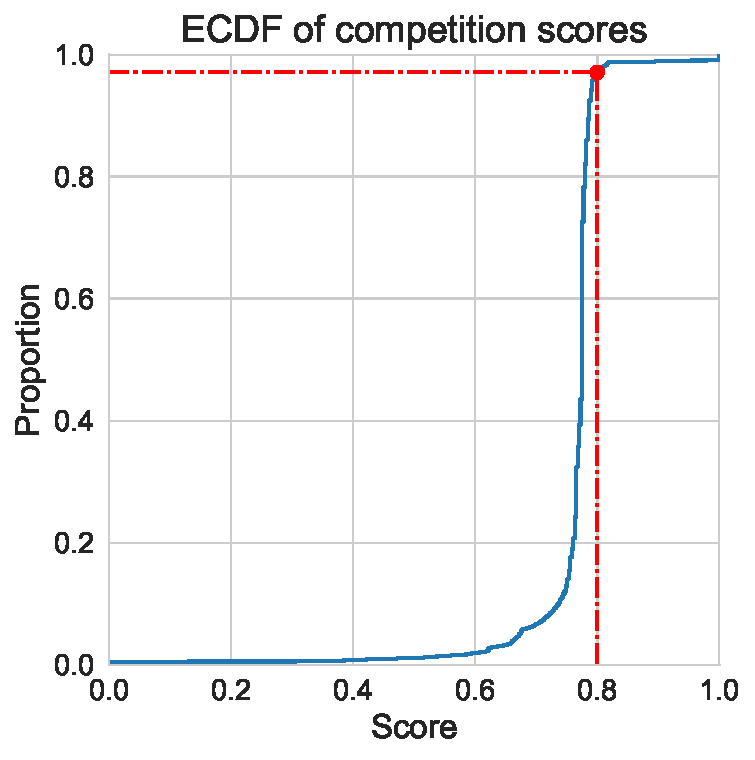
\includegraphics[width=0.5\textwidth]{leaderboard_scores_ecdf}
	\caption{Leaderboard Scores ECDF}
	\label{pic:leaderboard_scores_ecdf}
\end{figure}

There are several solutions with a score equal to 1.0. These solutions 
are marked with a red arrow in the figure \ref{pic:leaderboard_scores_kde}. 
Have authors reached perfection?

\begin{figure}[!ht]
	\centering
	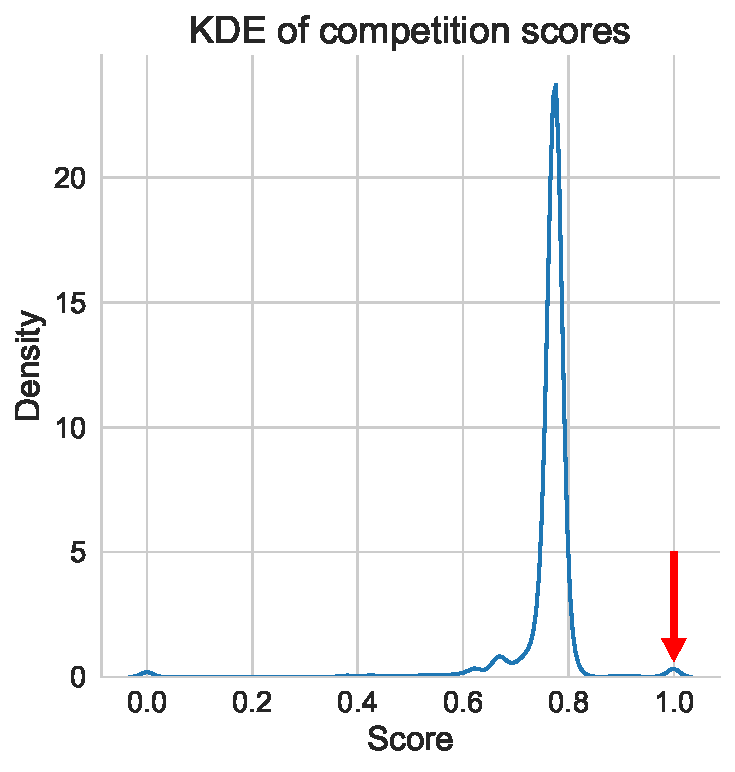
\includegraphics[width=0.5\textwidth]{leaderboard_scores_kde}
	\caption{Leaderboard Scores KDE}
	\label{pic:leaderboard_scores_kde}
\end{figure}

I guess, this solutions appears, because there is an exact solution on
\href{https://github.com/thisisjasonjafari/my-datascientise-handcode/raw/master/005-datavisualization/titanic.csv}
{GitHub}. Possibly it is the data extracted from 
\href{https://www.encyclopedia-titanica.org/titanic-survivors/}
{Encyclopedia Titanica}\cite{encyclopedia_titanica} or from
\href{https://www.openml.org/search?type=data&sort=runs&id=40945&status=active}
{OpenML}~\cite{openml_titanic}. Some authors in their notebooks honestly warn 
other users about the existence of such a possibility, for example, 
\href{https://www.kaggle.com/code/suzukifelipe/how-to-be-a-top-lb-explained-for-beginners/notebook?scriptVersionId=99817039}{this one}
\cite{perfection_explanation}.


\section{Data Dictionary}
\begin{enumerate}
	\item \textbf{PassengerId} -- Passenger ID.
	\item \textbf{Survived} -- Survival:
	\begin{itemize}
	    \item 0 = No, 
	    \item 1 = Yes.
	\end{itemize}
	\item \textbf{Pclass} -- Ticket class:
	\begin{itemize}	
	    \item 1 = 1st, 
	    \item 2 = 2nd, 
	    \item 3 = 3rd.
    \end{itemize}
	\item \textbf{Name} -- Passanger's name, for example, "Braund, 
	Mr. Owen Harris".
	\item \textbf{Sex} -- Gender:
	\begin{itemize}
	    \item male,
	    \item female.
	\end{itemize}
	\item \textbf{Age} -- Age in years, for example 38.0.
	\item \textbf{SibSp} -- Number of siblings or spouses aboard the Titanic.
	\item \textbf{Parch} -- Number of parents or children aboard the Titanic.
	\item \textbf{Ticket} -- Ticket number, for example, A/5 21171.
	\item \textbf{Fare} -- Passenger fare, for ecample, 71.2833.
	\item \textbf{Cabin} -- Cabin number, for example, C85.
	\item \textbf{Embarked} -- Port of Embarkation:
	\begin{itemize}
	    \item C = Cherbourg,
	    \item Q = Queenstown,
	    \item S = Southampton.
	\end{itemize}
\end{enumerate}


\subsection{Features}
PassengerId, Pclass, Name, Sex, Age, SibSp, Parch, Ticket, Fare, Cabin, 
\\Embarked


\subsection{Target}
Survived


\subsection{Variable Notes}
\begin{itemize}
	\item \textbf{Pclass}: socio-economic status
		\begin{itemize}
		    \item 1st = Upper
		    \item 2nd = Middle
		    \item 3rd = Lower
		\end{itemize}
	\item \textbf{Age}: Age is fractional if less than 1. If the age is 
	estimated, is it in the form of xx.5
	\item \textbf{SibSp} number of sibling/spouses aboard the Titanic
		\begin{itemize}
		    \item sibling = brother, sister, stepbrother, stepsister
		    \item spouse = husband, wife (mistresses and fiancés were 
		    ignored)
		\end{itemize}
	\item \textbf{Parch} number of parents (mother, father)/children 
	(daughter, son, stepdauter, stepson) aboard the Titanic. Some 
	children travelled only with a nanny, therefore \textbf{Parch}=0 for 
	them.
\end{itemize}


\section{File Paths}
\begin{itemize}
	\item \textbf{training set}: \url{../datasets/train.csv}
	\item \textbf{test set}: \url{../datasets/test.csv}
	\item \textbf{example of a submission file}:
	\url{../datasets/gender_submission.csv}
\end{itemize}


\section{Assumptions}
Women were more likely to survive than men.